\documentclass[../main.tex]{subfiles}
\section{Contagion on the Model}

As equation (\ref{local_p_comp}) shows, price contagion depends, via $P(\matr{Y})$, on the matrix $(2\matr{I} + \matr{G})^{-1}$ which we can define as the ``bargaining power'' matrix, since it allocates the excess revenues, $\Delta_t$, among providers in the network. For example, in the case of a positive demand shock and an increase in the local price of electricity of a given node, the excess demand will be partially absorbed by all other nodes in the network which, in turn, causes a contagion of local price hikes. Hence, the spread of the price hikes depends on the bargaining power of nodes in the matrix. Sticking with our example, if $X_{i, t}$ increases suddenly, $\Delta^{(i, j)}_t$ increases, and the cross-border prices across the network increase by
\begin{equation*}
    (2\matr{I} + \matr{G})^{-1}_{(k, l), (i, j)}
\end{equation*}

This implies that a provider with a stronger bargaining position reacts more strongly to price changes, captures higher revenue, which leads to higher prices in the local market. Intuitevely it also follows that a denser network, which results in a more equal distirbution of bargaining power, leads to lower revenues for providers and lower price hikes. To formalize this, consider the entry $(i, j)$ in $P(\Y_t)$,

\begin{equation*}
    P^{(i, j)}_t = \frac{\sum_{(l, m) \in E} \Delta^{(l, m)}_t \cdot (2\matr{I} + \matr{G})^{-1}_{(i, j), (l, m)}}{Y^{(i, j)}_t},
\end{equation*}

where $\sum_{(l, m) \in E}$ is a summation over the row $(i, j)$ of $(2\matr{I} + \matr{G})^{-1}$. Now assume there is some demand shock in a node $k$. We would like to understand the effect this has on prices today, $P^{(i, j)}_t$, and tomorrow, $P^{(i, j)}_{t+1}$. To do so we can first note that the current traded quantity between the two nodes $i$ and $j$, $Y^{(i, j)}_t$, is not affected by a change in $X_{k, t}$ since it will only affect current prices and future quantities between $i$ and $j$ ($X_{k, t} \rightarrow P^{(i, j)}_{t} \rightarrow p_{i, t} \rightarrow X_{i, t+1}$), hence $\partial Y^{(i, j)}_t / \partial X_{k, t} = 0$. This is of course not true for $Y^{(i, j)}_{t+1}$. Now,

\begin{equation}
    \begin{split}
        \frac{P^{(i, j)}_{t}}{\partial X_{k, t}} &= \frac{1}{Y^{(i, j)}_t} \left( p_{k, t} \cdot \sum_{(k, m) \in E} (2\matr{I} + \matr{G})^{-1}_{(i, j), (k, m)} - p_{k, t} \cdot \sum_{(l, k) \in E} (2\matr{I} + \matr{G})^{-1}_{(i, j), (l, k)} \right) \\
        &= \frac{p_{k, t}}{Y^{(i, j)}_t} \underbrace{\left(\sum_{(k, m) \in E} (2\matr{I} + \matr{G})^{-1}_{(i, j), (k, m)} -  \sum_{(l, k) \in E} (2\matr{I} + \matr{G})^{-1}_{(i, j), (l, k)} \right)}_{\text{influence of $k$ on the network}}
    \end{split}
\end{equation}

\begin{figure}[!ht]
    \centering
    % First row
    \begin{subfigure}[t]{.4\textwidth}
        \centering
        \includegraphics[width=\linewidth]{\bargpath/line.pdf}
        \caption{On a sequential graph} \label{fig:linepower}
    \end{subfigure}
    \hfill
    \begin{subfigure}[t]{.4\textwidth}
        \centering
        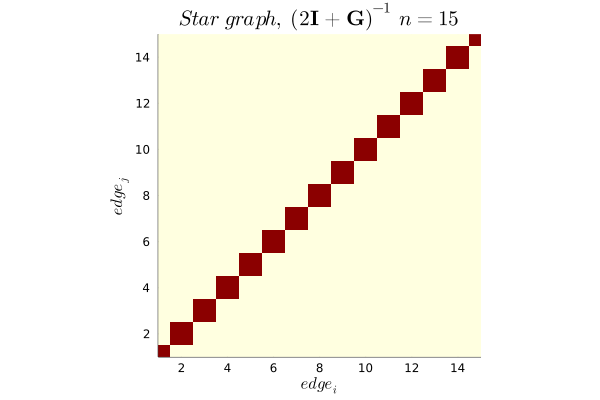
\includegraphics[width=\linewidth]{\bargpath/star.pdf}
        \caption{On a star graph} \label{fig:starpower}
    \end{subfigure}


    \medskip

    % Second row
    \begin{subfigure}[t]{.4\textwidth}
        \centering
        \includegraphics[width=\linewidth]{\bargpath/binarytree.pdf}
        \caption{On a binary tree} \label{fig:btreepower}
    \end{subfigure}
    \hfill
    \begin{subfigure}[t]{.4\textwidth}
        \centering
        \includegraphics[width=\linewidth]{\bargpath/complete.pdf}
        \caption{On a complete} \label{fig:completepower}
    \end{subfigure}
    \caption{Network influence} \label{fig:influence}
\end{figure}

This influence value gives a first order approximation of the effect on the network of a demand shock in a given node. In Figure \ref{fig:influence} I plotted the influence of each node on different graphs that will be used in the simulation. It is wise to stop here with the analytical work given the complex behaviour of $P^{(i, j)}_{t + 1} / \partial X_{k, t}$, hence in the next section I will look at contagion by means of simulation.

\subsection{Contagion simulation}


\begin{figure}[!ht]
    \centering
    \begin{minipage}{.5\textwidth}
        \centering
        \includegraphics[width=\linewidth]{\plotpath/line/pricesupply.pdf}
        \caption{Line}
        \label{fig:lineprice}
    \end{minipage}%
    \begin{minipage}{.5\textwidth}
        \centering
        \includegraphics[width=\linewidth]{\plotpath/smallstar/pricesupply.pdf}
        \caption{Small star}
        \label{fig:smallstarprice}
    \end{minipage}
\end{figure}